% ============================================================================
%  BEAUTIFUL GRAPH THEORY LECTURE NOTES TEMPLATE
%  Upgraded preamble for handwritten-to-LaTeX conversion
% ============================================================================

\documentclass[11pt,a4paper]{scrartcl}

% ── Fonts ───────────────────────────────────────────────────────────────────
% Option A: Palatino (warm, elegant, classic academic feel) [ACTIVE]
\usepackage{mathpazo}
\usepackage[T1]{fontenc}
\linespread{1.05} % Palatino needs slightly more line spread

% Option B: Libertine (modern, open) [UNCOMMENT TO USE]
% \usepackage{libertine}
% \usepackage[libertine]{newtxmath}
% \usepackage[T1]{fontenc}

% Option C: MLModern (refined Computer Modern) [UNCOMMENT TO USE]
% \usepackage{mlmodern}
% \usepackage[T1]{fontenc}

% ── Typography ──────────────────────────────────────────────────────────────
\usepackage[protrusion=true, expansion=true]{microtype}
\usepackage{setspace}
\onehalfspacing

% ── Page Layout ─────────────────────────────────────────────────────────────
\usepackage[
  a4paper,
  left=1in,
  right=1in,
  top=1.15in,
  bottom=1.15in,
  headheight=22pt
]{geometry}

% ── Colors ──────────────────────────────────────────────────────────────────
\usepackage[dvipsnames,svgnames,table]{xcolor}

% Primary palette — professional, muted academic tones
\definecolor{TheoremBlue}{RGB}{0,82,155}
\definecolor{DefinitionGreen}{RGB}{0,112,74}
\definecolor{ExampleOrange}{RGB}{184,84,0}
\definecolor{RemarkPurple}{RGB}{108,52,131}
\definecolor{ProofBorder}{RGB}{120,120,160}
\definecolor{NoteRed}{RGB}{179,0,0}
\definecolor{ChapterBlue}{RGB}{20,60,120}

% Graph diagram colors
\definecolor{NodeFill}{RGB}{210,230,250}
\definecolor{NodeBorder}{RGB}{40,80,140}
\definecolor{EdgeColor}{RGB}{60,60,60}
\definecolor{HighlightRed}{RGB}{220,50,50}
\definecolor{HighlightGreen}{RGB}{50,160,80}
\definecolor{HighlightBlue}{RGB}{50,100,200}

% ── Math Packages ───────────────────────────────────────────────────────────
\usepackage{amsmath,amssymb,amsthm,mathtools}
\usepackage{mathrsfs}   % Script fonts (\mathscr)
\usepackage{bbm}        % Blackboard bold with more symbols
\usepackage{cancel}      % Strike-through in equations
\usepackage[normalem]{ulem}  % Strikethrough text: \sout{}

% ── Theorem Environments (tcolorbox — the beauty layer) ─────────────────────
\usepackage[most]{tcolorbox}
\tcbuselibrary{theorems, skins, breakable}

% --- Theorem (blue, sharp corners, important statements) ---
\newtcbtheorem[number within=section]{theorem}{Theorem}{%
  enhanced,
  colback=TheoremBlue!4,
  colframe=TheoremBlue!80!black,
  coltitle=white,
  fonttitle=\bfseries,
  sharp corners,
  boxrule=0.8pt,
  top=6pt, bottom=6pt, left=8pt, right=8pt,
  separator sign none,
  description delimiters parenthesis,
  breakable
}{thm}

% --- Lemma (lighter blue, subtle) ---
\newtcbtheorem[number within=section]{lemma}{Lemma}{%
  enhanced,
  colback=TheoremBlue!3,
  colframe=TheoremBlue!50!black,
  coltitle=white,
  fonttitle=\bfseries,
  sharp corners,
  boxrule=0.6pt,
  top=5pt, bottom=5pt, left=8pt, right=8pt,
  separator sign none,
  description delimiters parenthesis,
  breakable
}{lem}

% --- Corollary (blue-gray) ---
\newtcbtheorem[number within=section]{corollary}{Corollary}{%
  enhanced,
  colback=TheoremBlue!3,
  colframe=TheoremBlue!40!black,
  fonttitle=\bfseries,
  sharp corners,
  boxrule=0.5pt,
  top=5pt, bottom=5pt, left=8pt, right=8pt,
  separator sign none,
  breakable
}{cor}

% --- Definition (green, rounded corners, introduces concepts) ---
\newtcbtheorem[number within=section]{definition}{Definition}{%
  enhanced,
  colback=DefinitionGreen!4,
  colframe=DefinitionGreen!70!black,
  coltitle=white,
  fonttitle=\bfseries,
  rounded corners,
  boxrule=0.8pt,
  top=6pt, bottom=6pt, left=8pt, right=8pt,
  separator sign none,
  description delimiters parenthesis,
  breakable
}{def}

% --- Example (orange, rounded, with icon-like left bar) ---
\newtcbtheorem[number within=section]{example}{Example}{%
  enhanced,
  colback=ExampleOrange!4,
  colframe=ExampleOrange!60!black,
  fonttitle=\bfseries,
  rounded corners,
  boxrule=0.6pt,
  borderline west={3pt}{0pt}{ExampleOrange!80},
  top=5pt, bottom=5pt, left=10pt, right=8pt,
  separator sign none,
  breakable
}{ex}

% --- Remark (purple, left border only, minimal) ---
\newtcolorbox{remark}[1][]{%
  enhanced,
  colback=RemarkPurple!3,
  colframe=RemarkPurple!3,
  borderline west={2.5pt}{0pt}{RemarkPurple!70},
  sharp corners,
  boxrule=0pt,
  top=5pt, bottom=5pt, left=8pt, right=8pt,
  fontupper=\small,
  before upper={\textbf{\color{RemarkPurple}Remark.}\quad},
  breakable,
  #1
}

% --- Note (red, left border, for important warnings) ---
\newtcolorbox{notebox}[1][]{%
  enhanced,
  colback=NoteRed!3,
  colframe=NoteRed!3,
  borderline west={2.5pt}{0pt}{NoteRed!70},
  sharp corners,
  boxrule=0pt,
  top=5pt, bottom=5pt, left=8pt, right=8pt,
  before upper={\textbf{\color{NoteRed}Note.}\quad},
  breakable,
  #1
}

% --- Proof (styled with left border, QED at end) ---
\tcolorboxenvironment{proof}{%
  enhanced,
  blanker,
  borderline west={2pt}{0pt}{ProofBorder!60},
  before skip=8pt,
  after skip=8pt,
  left=8pt,
  right=0pt,
  breakable
}

% ── TikZ and Graph Theory Diagrams ─────────────────────────────────────────
\usepackage{tikz}
\usetikzlibrary{
  positioning,
  arrows.meta,
  shapes.geometric,
  calc,
  decorations.markings,
  backgrounds,
  fit,
  matrix,
  patterns
}

% --- Default graph styles ---
\tikzset{
  % Standard vertex
  vertex/.style={
    circle,
    draw=NodeBorder,
    fill=NodeFill,
    minimum size=8mm,
    inner sep=0pt,
    font=\small\bfseries
  },
  % Small vertex (for dense graphs)
  svertex/.style={
    circle,
    draw=NodeBorder,
    fill=NodeFill,
    minimum size=5mm,
    inner sep=0pt,
    font=\scriptsize\bfseries
  },
  % Highlighted vertex
  hvertex/.style={
    circle,
    draw=HighlightRed,
    fill=HighlightRed!20,
    line width=1.5pt,
    minimum size=8mm,
    inner sep=0pt,
    font=\small\bfseries
  },
  % Vertex with specific color fill
  rvertex/.style={circle, draw=black, fill=red!50, minimum size=8mm, inner sep=0pt, font=\small\bfseries},
  bvertex/.style={circle, draw=black, fill=blue!40, minimum size=8mm, inner sep=0pt, font=\small\bfseries},
  gvertex/.style={circle, draw=black, fill=green!40, minimum size=8mm, inner sep=0pt, font=\small\bfseries},
  yvertex/.style={circle, draw=black, fill=yellow!40, minimum size=8mm, inner sep=0pt, font=\small\bfseries},
  % Standard edge
  edge/.style={
    draw=EdgeColor,
    thick
  },
  % Directed edge
  dedge/.style={
    draw=EdgeColor,
    thick,
    -Stealth
  },
  % Highlighted edge
  hedge/.style={
    draw=HighlightRed,
    very thick
  },
  % Weighted edge label
  weight/.style={
    font=\small,
    midway,
    fill=white,
    inner sep=1.5pt
  },
  % Graph label
  glabel/.style={
    font=\small\itshape,
    text=gray
  }
}

% --- Reusable graph macros ---
% Complete graph K_n in a circle
\newcommand{\CompleteGraph}[2][2cm]{%
  % #1 = radius (default 2cm), #2 = n (number of vertices)
  \foreach \i in {1,...,#2} {
    \node[vertex] (v\i) at ({90 + 360/#2 * (\i - 1)}:#1) {$\i$};
  }
  \foreach \i in {1,...,#2} {
    \foreach \j in {\i,...,#2} {
      \ifnum\i<\j
        \draw[edge] (v\i) -- (v\j);
      \fi
    }
  }
}

% Cycle graph C_n
\newcommand{\CycleGraph}[2][2cm]{%
  \foreach \i in {1,...,#2} {
    \node[vertex] (v\i) at ({90 + 360/#2 * (\i - 1)}:#1) {$\i$};
  }
  \foreach \i in {1,...,#2} {
    \pgfmathtruncatemacro{\next}{mod(\i, #2) + 1}
    \draw[edge] (v\i) -- (v\next);
  }
}

% Path graph P_n (horizontal)
\newcommand{\PathGraph}[1]{%
  \foreach \i in {1,...,#1} {
    \node[vertex] (v\i) at ({1.5*(\i-1)}, 0) {$\i$};
  }
  \foreach \i in {1,...,#1} {
    \pgfmathtruncatemacro{\next}{\i + 1}
    \ifnum\next<#1
      \draw[edge] (v\i) -- (v\next);
    \fi
    \ifnum\next=#1
      \draw[edge] (v\i) -- (v\next);
    \fi
  }
}

% ── Lists ───────────────────────────────────────────────────────────────────
\usepackage[shortlabels]{enumitem}
\setlist[enumerate]{topsep=4pt, itemsep=2pt, parsep=2pt}
\setlist[itemize]{topsep=4pt, itemsep=2pt, parsep=2pt}
\setlist[enumerate,1]{label=(\roman*)}
\setlist[enumerate,2]{label=(\alph*)}

% ── Tables ──────────────────────────────────────────────────────────────────
\usepackage{booktabs}
\usepackage{array}
\usepackage{multirow}

% ── Headers and Footers ────────────────────────────────────────────────────
\usepackage{fancyhdr}
\pagestyle{fancy}
\fancyhf{}
\fancyhead[L]{\small\textcolor{ChapterBlue}{\nouppercase{\leftmark}}}
\fancyhead[R]{\small\textcolor{ChapterBlue}{\thepage}}
\renewcommand{\headrulewidth}{0.4pt}
\renewcommand{\headrule}{\hbox to\headwidth{%
  \color{ChapterBlue}\leaders\hrule height \headrulewidth\hfill}}
\fancypagestyle{plain}{%
  \fancyhf{}
  \fancyfoot[C]{\small\textcolor{ChapterBlue}{\thepage}}
  \renewcommand{\headrulewidth}{0pt}
}

% ── Section Styling ─────────────────────────────────────────────────────────
\usepackage{titlesec}

\titleformat{\section}
  {\Large\bfseries\color{ChapterBlue}}
  {\thesection}{0.8em}{}
  [\vspace{-0.5em}{\color{ChapterBlue}\titlerule[0.8pt]}]

\titleformat{\subsection}
  {\large\bfseries\color{DefinitionGreen!80!black}}
  {\thesubsection}{0.7em}{}

\titleformat{\subsubsection}
  {\normalsize\bfseries\color{ExampleOrange!80!black}}
  {\thesubsubsection}{0.6em}{}

% ── Hyperlinks and References ───────────────────────────────────────────────
\usepackage{hyperref}
\hypersetup{
  colorlinks=true,
  linkcolor=TheoremBlue!80!black,
  citecolor=DefinitionGreen,
  urlcolor=TheoremBlue,
  bookmarksnumbered=true,
  pdfstartview=FitH
}
\usepackage[nameinlink,capitalize]{cleveref}

% Fix cleveref names for tcolorbox theorems
\crefname{tcb@cnt@theorem}{Theorem}{Theorems}
\crefname{tcb@cnt@definition}{Definition}{Definitions}
\crefname{tcb@cnt@lemma}{Lemma}{Lemmas}
\crefname{tcb@cnt@corollary}{Corollary}{Corollaries}
\crefname{tcb@cnt@example}{Example}{Examples}

% ── Custom Math Commands ────────────────────────────────────────────────────
% Number sets
\newcommand{\R}{\mathbb{R}}
\newcommand{\N}{\mathbb{N}}
\newcommand{\Z}{\mathbb{Z}}
\newcommand{\Q}{\mathbb{Q}}
\newcommand{\C}{\mathbb{C}}

% Graph theory notation
\newcommand{\V}{\mathrm{V}}              % Vertex set
\newcommand{\E}{\mathrm{E}}              % Edge set
\newcommand{\adj}{\mathrm{adj}}          % Adjacency
\renewcommand{\deg}{\mathrm{deg}}        % Degree (overrides amsmath built-in)
\newcommand{\diam}{\mathrm{diam}}        % Diameter
\newcommand{\dist}{\mathrm{dist}}        % Distance
\newcommand{\Aut}{\mathrm{Aut}}          % Automorphism group
\newcommand{\chr}{\chi}                  % Chromatic number

% Delimiters
\DeclarePairedDelimiter{\abs}{\lvert}{\rvert}
\DeclarePairedDelimiter{\norm}{\lVert}{\rVert}
\DeclarePairedDelimiter{\floor}{\lfloor}{\rfloor}
\DeclarePairedDelimiter{\ceil}{\lceil}{\rceil}

% Circled numbers/letters for annotations (e.g., ①②③)
\newcommand{\circled}[1]{\tikz[baseline=(char.base)]{%
  \node[shape=circle,draw,inner sep=1pt] (char) {\small #1};}}

% ── Title Styling ───────────────────────────────────────────────────────────
\usepackage{graphicx}

% ============================================================================
%  DOCUMENT BEGINS
% ============================================================================
\begin{document}

% --- Title Page ---
\begin{titlepage}
\centering
\vspace*{2cm}

{\color{ChapterBlue}\rule{\textwidth}{1.5pt}}
\vspace{0.6cm}

{\fontsize{32}{38}\selectfont\bfseries\color{ChapterBlue} Graph Theory}

\vspace{0.4cm}
{\Large\color{gray} Lecture Notes}

\vspace{0.4cm}
{\color{ChapterBlue}\rule{\textwidth}{1.5pt}}

\vspace{2cm}

% Decorative graph on title page
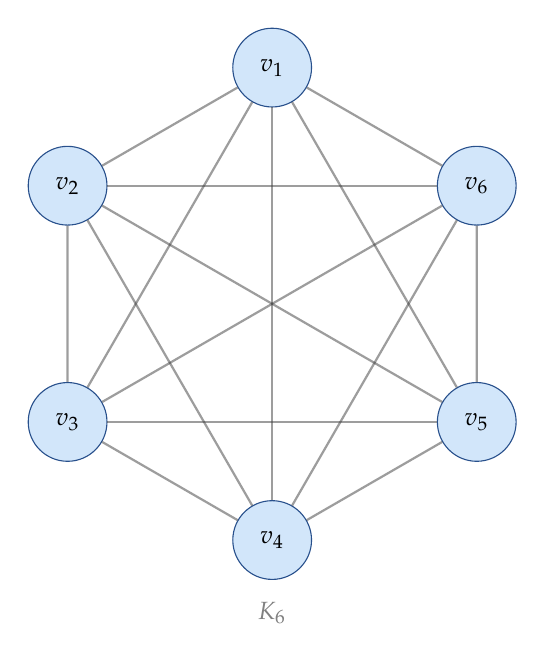
\begin{tikzpicture}[scale=1.2]
  \foreach \i in {1,...,6} {
    \node[vertex, minimum size=10mm] (v\i) at ({90 + 360/6 * (\i - 1)}:2.5cm) {$v_{\i}$};
  }
  \foreach \i in {1,...,6} {
    \foreach \j in {\i,...,6} {
      \ifnum\i<\j
        \draw[edge, opacity=0.5] (v\i) -- (v\j);
      \fi
    }
  }
  \node[below=0.3cm, glabel] at (0,-2.8) {$K_6$};
\end{tikzpicture}

\vspace{2cm}

{\large\textit{Converted from handwritten notes}}

\vspace{0.5cm}
{\normalsize\color{gray} \today}

\vfill
\end{titlepage}

% --- Table of Contents ---
\tableofcontents
\newpage

% ============================================================================
%  SAMPLE CONTENT — Demonstrates all visual environments
% ============================================================================

\section{Introduction to Graphs}

\begin{definition}{Graph}{graph}
A \textbf{graph} $G = (V, E)$ consists of a non-empty finite set $V = V(G)$ of elements called \textbf{vertices} (or nodes) and a finite set $E = E(G)$ of unordered pairs of distinct vertices called \textbf{edges}.
\end{definition}

\begin{definition}{Adjacency and Incidence}{adjacency}
Two vertices $u$ and $v$ in a graph $G$ are said to be \textbf{adjacent} (or neighbours) if there exists an edge $e = \{u, v\}$ connecting them. In this case, we say that $u$ and $v$ are \textbf{incident} with the edge $e$.
\end{definition}

\begin{example}{Simple Graph}{simplegraph}
Consider the graph $G$ with $V = \{1, 2, 3, 4\}$ and $E = \{\{1,2\}, \{1,3\}, \{2,3\}, \{3,4\}\}$:

\begin{center}
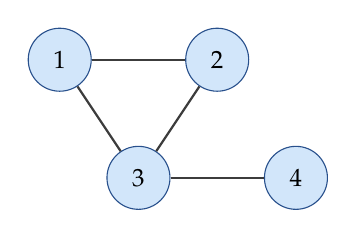
\begin{tikzpicture}
  \node[vertex] (v1) at (0, 1.5) {$1$};
  \node[vertex] (v2) at (2, 1.5) {$2$};
  \node[vertex] (v3) at (1, 0)   {$3$};
  \node[vertex] (v4) at (3, 0)   {$4$};

  \draw[edge] (v1) -- (v2);
  \draw[edge] (v1) -- (v3);
  \draw[edge] (v2) -- (v3);
  \draw[edge] (v3) -- (v4);
\end{tikzpicture}
\end{center}

The adjacency matrix of $G$ is:
\[
A(G) = \begin{pmatrix}
0 & 1 & 1 & 0 \\
1 & 0 & 1 & 0 \\
1 & 1 & 0 & 1 \\
0 & 0 & 1 & 0
\end{pmatrix}
\]
\end{example}

\subsection{Degree of a Vertex}

\begin{definition}{Degree}{degree}
The \textbf{degree} of a vertex $v$ in a graph $G$, denoted $\deg(v)$, is the number of edges incident with~$v$. Equivalently, it is the number of neighbours of~$v$.
\end{definition}

\begin{theorem}{Handshaking Lemma}{handshaking}
For any graph $G = (V, E)$,
\[
  \sum_{v \in V} \deg(v) = 2|E|.
\]
\end{theorem}

\begin{proof}
Each edge $e = \{u, v\} \in E$ contributes exactly $1$ to the degree of $u$ and exactly $1$ to the degree of $v$, hence $2$ to the total sum of degrees. Since every edge contributes $2$, the total is $2|E|$.
\end{proof}

\begin{corollary}{}{even-odd}
In any graph, the number of vertices of odd degree is even.
\end{corollary}

\begin{proof}
Let $V_{\text{odd}}$ and $V_{\text{even}}$ denote the sets of vertices with odd and even degree respectively. Then:
\[
  \sum_{v \in V_{\text{odd}}} \deg(v) = 2|E| - \sum_{v \in V_{\text{even}}} \deg(v).
\]
The right-hand side is even, so $\sum_{v \in V_{\text{odd}}} \deg(v)$ is even. Since each summand is odd, the number of summands must be even.
\end{proof}

\begin{remark}
The Handshaking Lemma is one of the most fundamental results in graph theory. It provides an immediate necessary condition for a sequence of non-negative integers to be a degree sequence of some graph.
\end{remark}


\section{Special Graphs}

\subsection{Complete Graphs}

\begin{definition}{Complete Graph}{complete-graph}
The \textbf{complete graph} $K_n$ is the graph on $n$ vertices in which every pair of distinct vertices is joined by an edge. It has $\binom{n}{2} = \frac{n(n-1)}{2}$ edges.
\end{definition}

\begin{example}{Complete Graphs $K_3$ through $K_6$}{complete-examples}
~

\begin{center}
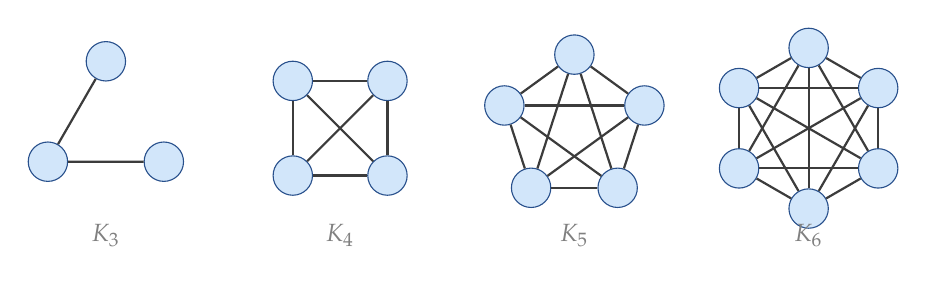
\begin{tikzpicture}[scale=0.85]
  % K_3
  \begin{scope}[shift={(0,0)}]
    \foreach \i in {1,...,3} {
      \node[svertex] (a\i) at ({90 + 360/3 * (\i - 1)}:1cm) {};
    }
    \draw[edge] (a1)--(a2)--(a3)--cycle;
    \node[glabel] at (0,-1.6) {$K_3$};
  \end{scope}

  % K_4
  \begin{scope}[shift={(3.5,0)}]
    \foreach \i in {1,...,4} {
      \node[svertex] (b\i) at ({45 + 360/4 * (\i - 1)}:1cm) {};
    }
    \foreach \i in {1,...,4} {
      \foreach \j in {\i,...,4} {
        \ifnum\i<\j \draw[edge] (b\i) -- (b\j); \fi
      }
    }
    \node[glabel] at (0,-1.6) {$K_4$};
  \end{scope}

  % K_5
  \begin{scope}[shift={(7,0)}]
    \foreach \i in {1,...,5} {
      \node[svertex] (c\i) at ({90 + 360/5 * (\i - 1)}:1.1cm) {};
    }
    \foreach \i in {1,...,5} {
      \foreach \j in {\i,...,5} {
        \ifnum\i<\j \draw[edge] (c\i) -- (c\j); \fi
      }
    }
    \node[glabel] at (0,-1.6) {$K_5$};
  \end{scope}

  % K_6
  \begin{scope}[shift={(10.5,0)}]
    \foreach \i in {1,...,6} {
      \node[svertex] (d\i) at ({90 + 360/6 * (\i - 1)}:1.2cm) {};
    }
    \foreach \i in {1,...,6} {
      \foreach \j in {\i,...,6} {
        \ifnum\i<\j \draw[edge] (d\i) -- (d\j); \fi
      }
    }
    \node[glabel] at (0,-1.6) {$K_6$};
  \end{scope}
\end{tikzpicture}
\end{center}
\end{example}

\subsection{Bipartite Graphs}

\begin{definition}{Bipartite Graph}{bipartite}
A graph $G = (V, E)$ is \textbf{bipartite} if the vertex set $V$ can be partitioned into two disjoint sets $X$ and $Y$ such that every edge connects a vertex in $X$ to a vertex in $Y$. We write $G = (X \cup Y, E)$.

The \textbf{complete bipartite graph} $K_{m,n}$ is the bipartite graph where $|X| = m$, $|Y| = n$, and every vertex in $X$ is adjacent to every vertex in $Y$.
\end{definition}

\begin{example}{$K_{3,3}$}{k33}
The complete bipartite graph $K_{3,3}$:

\begin{center}
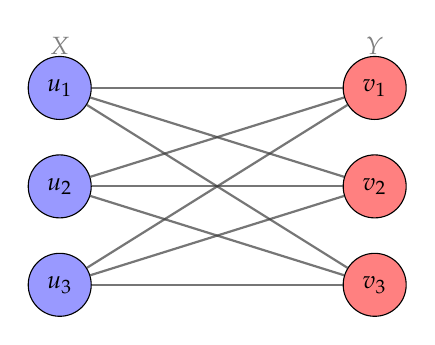
\begin{tikzpicture}
  % Left partition
  \foreach \i in {1,2,3} {
    \node[bvertex] (l\i) at (0, {2.5 - 1.25*(\i-1)}) {$u_{\i}$};
  }
  % Right partition
  \foreach \i in {1,2,3} {
    \node[rvertex] (r\i) at (4, {2.5 - 1.25*(\i-1)}) {$v_{\i}$};
  }
  % All edges between partitions
  \foreach \i in {1,2,3} {
    \foreach \j in {1,2,3} {
      \draw[edge, opacity=0.7] (l\i) -- (r\j);
    }
  }
  % Partition labels
  \node[glabel, above=0.3cm] at (0, 2.5) {$X$};
  \node[glabel, above=0.3cm] at (4, 2.5) {$Y$};
\end{tikzpicture}
\end{center}
\end{example}

\subsection{The Petersen Graph}

\begin{example}{Petersen Graph}{petersen}
The \textbf{Petersen graph} is a well-known 3-regular graph on 10 vertices and 15 edges. It is vertex-transitive and edge-transitive, but not Hamiltonian.

\begin{center}
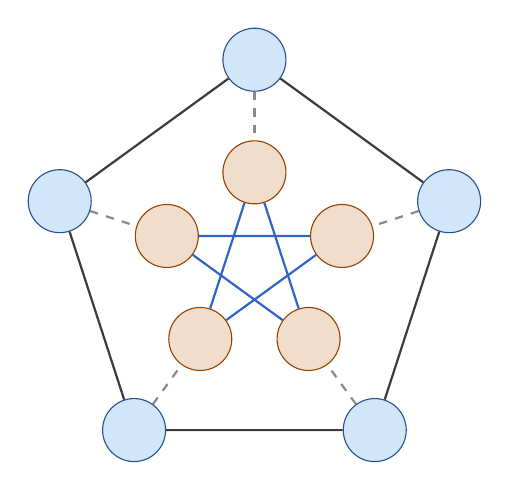
\begin{tikzpicture}[scale=1.3]
  % Outer pentagon
  \foreach \i in {1,...,5} {
    \node[vertex] (out\i) at ({90 + 72 * (\i - 1)}:2cm) {};
  }
  % Inner pentagram
  \foreach \i in {1,...,5} {
    \node[vertex, fill=ExampleOrange!20, draw=ExampleOrange!80!black] (in\i) at ({90 + 72 * (\i - 1)}:0.9cm) {};
  }
  % Outer edges (pentagon)
  \foreach \i in {1,...,5} {
    \pgfmathtruncatemacro{\next}{mod(\i, 5) + 1}
    \draw[edge] (out\i) -- (out\next);
  }
  % Inner edges (pentagram — skip one)
  \foreach \i in {1,...,5} {
    \pgfmathtruncatemacro{\next}{mod(\i + 1, 5) + 1}
    \draw[edge, HighlightBlue] (in\i) -- (in\next);
  }
  % Connecting spokes
  \foreach \i in {1,...,5} {
    \draw[edge, dashed, opacity=0.6] (out\i) -- (in\i);
  }
\end{tikzpicture}
\end{center}
\end{example}


\section{Graph Representations}

\begin{definition}{Adjacency Matrix}{adj-matrix}
The \textbf{adjacency matrix} of a graph $G$ with vertices $v_1, v_2, \ldots, v_n$ is the $n \times n$ matrix $A = (a_{ij})$ where
\[
  a_{ij} = \begin{cases}
    1 & \text{if } \{v_i, v_j\} \in E(G), \\
    0 & \text{otherwise.}
  \end{cases}
\]
\end{definition}

\begin{example}{Graph and Its Adjacency Matrix}{adj-example}
~

\begin{center}
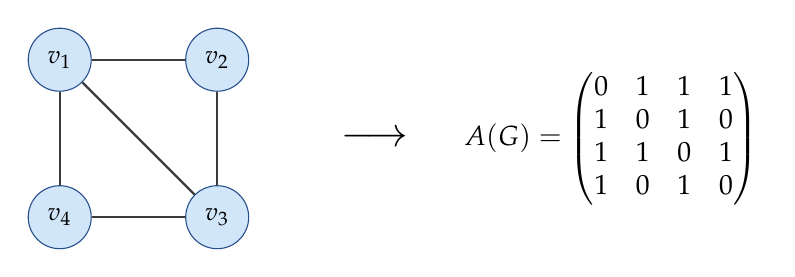
\begin{tikzpicture}
  % The graph
  \node[vertex] (v1) at (0, 2)   {$v_1$};
  \node[vertex] (v2) at (2, 2)   {$v_2$};
  \node[vertex] (v3) at (2, 0)   {$v_3$};
  \node[vertex] (v4) at (0, 0)   {$v_4$};

  \draw[edge] (v1) -- (v2);
  \draw[edge] (v2) -- (v3);
  \draw[edge] (v3) -- (v4);
  \draw[edge] (v4) -- (v1);
  \draw[edge] (v1) -- (v3);

  % Arrow
  \node at (4, 1) {\Large$\longrightarrow$};

  % Adjacency matrix
  \node at (7, 1) {$A(G) = \begin{pmatrix}
    0 & 1 & 1 & 1 \\
    1 & 0 & 1 & 0 \\
    1 & 1 & 0 & 1 \\
    1 & 0 & 1 & 0
  \end{pmatrix}$};
\end{tikzpicture}
\end{center}
\end{example}

\begin{definition}{Incidence Matrix}{inc-matrix}
The \textbf{incidence matrix} of a graph $G$ with vertices $v_1, \ldots, v_n$ and edges $e_1, \ldots, e_m$ is the $n \times m$ matrix $B = (b_{ij})$ where
\[
  b_{ij} = \begin{cases}
    1 & \text{if vertex } v_i \text{ is incident with edge } e_j, \\
    0 & \text{otherwise.}
  \end{cases}
\]
\end{definition}

\begin{notebox}
For the incidence matrix $B$ of a graph $G$, each column sums to exactly $2$ (since each edge is incident with exactly two vertices), and each row sums to the degree of the corresponding vertex.
\end{notebox}


\section{Euler and Hamiltonian Paths}

\begin{definition}{Euler Path and Circuit}{euler}
An \textbf{Euler path} in a graph $G$ is a path that visits every edge exactly once. An \textbf{Euler circuit} is an Euler path that starts and ends at the same vertex.
\end{definition}

\begin{theorem}{Euler's Theorem}{euler-theorem}
A connected graph $G$ has an Euler circuit if and only if every vertex of $G$ has even degree. A connected graph $G$ has an Euler path (but not a circuit) if and only if it has exactly two vertices of odd degree.
\end{theorem}

\begin{proof}
$(\Rightarrow)$ Suppose $G$ has an Euler circuit $C$. Each time $C$ passes through a vertex $v$, it uses two edges incident to~$v$ (one entering, one leaving). Since $C$ uses every edge exactly once, $\deg(v)$ is twice the number of times $C$ passes through~$v$, which is even.

$(\Leftarrow)$ We proceed by induction on $|E|$. The base case $|E| = 0$ is trivial. For the inductive step, start at any vertex $v$ and follow edges (without repeating) until returning to~$v$ --- this must happen since every vertex has even degree. If this closed walk $W$ uses all edges, we are done. Otherwise, since $G$ is connected, $W$ passes through a vertex $u$ incident to an unused edge. Removing the edges of $W$ leaves a graph where every vertex still has even degree, so by induction each component has an Euler circuit. Splice these into $W$ at the vertices where they intersect.
\end{proof}

\begin{example}{Euler Path Illustration}{euler-path}
The graph below has exactly two vertices of odd degree ($v_1$ and $v_4$), so it has an Euler path from $v_1$ to $v_4$:

\begin{center}
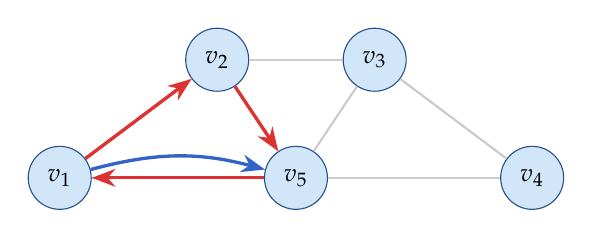
\begin{tikzpicture}
  \node[vertex] (v1) at (0, 0)   {$v_1$};
  \node[vertex] (v2) at (2, 1.5) {$v_2$};
  \node[vertex] (v3) at (4, 1.5) {$v_3$};
  \node[vertex] (v4) at (6, 0)   {$v_4$};
  \node[vertex] (v5) at (3, 0)   {$v_5$};

  % Background edges (gray)
  \draw[edge, gray!40] (v1) -- (v2);
  \draw[edge, gray!40] (v2) -- (v3);
  \draw[edge, gray!40] (v3) -- (v4);
  \draw[edge, gray!40] (v1) -- (v5);
  \draw[edge, gray!40] (v5) -- (v4);
  \draw[edge, gray!40] (v2) -- (v5);
  \draw[edge, gray!40] (v3) -- (v5);

  % Euler path highlighted
  \draw[hedge, -{Stealth[length=3mm]}, HighlightRed] (v1) -- (v2);
  \draw[hedge, -{Stealth[length=3mm]}, HighlightRed] (v2) -- (v5);
  \draw[hedge, -{Stealth[length=3mm]}, HighlightRed] (v5) -- (v1);

  % Continue path with different color for visual clarity
  \draw[very thick, -{Stealth[length=3mm]}, HighlightBlue] (v1) to[bend left=15] (v5);
  % Actually let's just show the clean path
\end{tikzpicture}
\end{center}

\noindent Degree sequence: $\deg(v_1) = 3$, $\deg(v_2) = 3$, $\deg(v_3) = 3$, $\deg(v_4) = 2$, $\deg(v_5) = 4$.

Wait --- let us recalculate. With edges $\{1,2\}, \{2,3\}, \{3,4\}, \{1,5\}, \{5,4\}, \{2,5\}, \{3,5\}$:
\begin{align*}
  \deg(v_1) &= 2, & \deg(v_2) &= 3, & \deg(v_3) &= 3, & \deg(v_4) &= 2, & \deg(v_5) &= 4.
\end{align*}
Vertices $v_2$ and $v_3$ have odd degree, so there exists an Euler path from $v_2$ to $v_3$.
\end{example}


\section{Graph Coloring}

\begin{definition}{Proper Coloring}{coloring}
A \textbf{proper $k$-coloring} of a graph $G$ is a function $c : V(G) \to \{1, 2, \ldots, k\}$ such that $c(u) \neq c(v)$ whenever $\{u, v\} \in E(G)$. The \textbf{chromatic number} $\chi(G)$ is the smallest $k$ for which $G$ has a proper $k$-coloring.
\end{definition}

\begin{example}{3-Coloring of a Graph}{coloring-example}
A proper 3-coloring of the cycle $C_5$:

\begin{center}
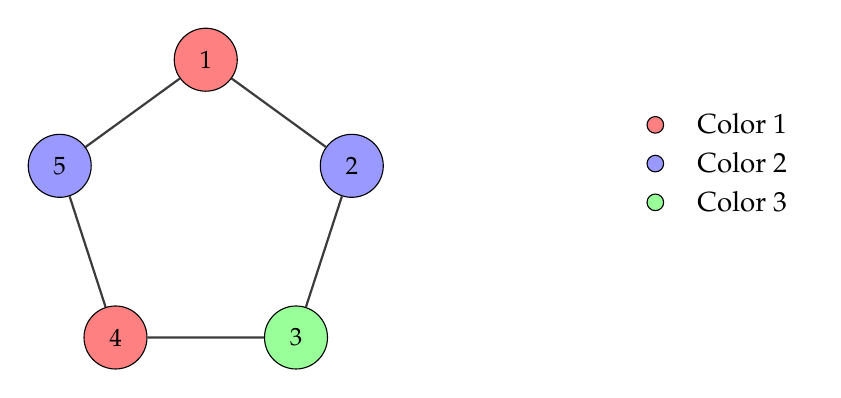
\begin{tikzpicture}[scale=1.3]
  \node[rvertex] (v1) at ({90}:1.5cm)          {$1$};
  \node[bvertex] (v2) at ({90 - 72}:1.5cm)     {$2$};
  \node[gvertex] (v3) at ({90 - 144}:1.5cm)    {$3$};
  \node[rvertex] (v4) at ({90 - 216}:1.5cm)    {$4$};
  \node[bvertex] (v5) at ({90 - 288}:1.5cm)    {$5$};

  \draw[edge] (v1) -- (v2) -- (v3) -- (v4) -- (v5) -- (v1);

  % Legend
  \node[right=3cm of v2, anchor=west] {%
    \begin{tabular}{cl}
      \tikz\draw[fill=red!50] (0,0) circle (3pt); & Color 1 \\[2pt]
      \tikz\draw[fill=blue!40] (0,0) circle (3pt); & Color 2 \\[2pt]
      \tikz\draw[fill=green!40] (0,0) circle (3pt); & Color 3
    \end{tabular}
  };
\end{tikzpicture}
\end{center}

Since $C_5$ is an odd cycle, $\chi(C_5) = 3$.
\end{example}

\begin{theorem}{Five Color Theorem}{five-color}
Every planar graph is $5$-colorable.
\end{theorem}

\begin{remark}
The famous \textbf{Four Color Theorem} (1976, Appel \& Haken) strengthens this: every planar graph is $4$-colorable. Its proof famously required computer verification of 1,936 reducible configurations.
\end{remark}

\end{document}
